\documentclass{ximera}

\usepackage{../OERLinearAlgebra}

\usepackage{mathtools}
\usepackage{tikz-3dplot}
\usetikzlibrary{shapes.geometric}
\usetikzlibrary{arrows}


\author{Paul Zachlin \and Anna Davis} \title{Describing Eigenvalues and Eigenvectors Algebraically and Geometrically} \license{CC-BY 4.0}


\begin{document}
\begin{abstract}
 We introduce the concepts of eigenvalues and eigenvectors of a matrix.
\end{abstract}
\maketitle

At several places in this course it has been valuable to restrict ourselves to square matrices, and we do so again when discussing eigenvalues and eigenvectors.  

In Theorem \ref{th:matrixtran} 
of Module LTR-M-0010, we proved that any $n \times n$  matrix induces a linear transformation from $\RR^n$ to itself.  For our first few examples, let us consider the case $n = 2$. 

\begin{initprob}\label{init:eignintro}
Let $A=\begin{bmatrix} 2& 1\\ 1&2
\end{bmatrix}$.  The following animation helps us to visualize the matrix transformation associated with $A$.

\begin{center}
    \geogebra{ub4kqvmz}{800}{600} 
  \end{center}

Given a vector $\vec{x}$ in $\RR^2$, the vector $A\vec{x}$ is also in $\RR^2$.  For many vectors, $A\vec{x}$ will not be pointing in the same direction as $\vec{x}$.  This is the case for any of the gray vectors in the animation, as we can see that $A\vec{x}$ points in a different direction than $\vec{x}$.  But if we look at the red vectors (vectors parallel to $\begin{bmatrix}-1\\1\end{bmatrix}$), we notice that they appear unchanged in magnitude and direction.  Such vectors are sometimes called \dfn{fixed vectors} of $A$.

Looking next at the blue vectors (vectors parallel to $\begin{bmatrix}1\\1\end{bmatrix}$), we observe that the magnitudes of the vectors are changed, but the direction in which the blue vectors point is unchanged by this linear transformation.  
\end{initprob}

In Exploration Problem \ref{init:eignintro} we found that certain vectors do not change direction under the linear transformation induced by matrix $A$.  Such vectors are examples of \dfn{eigenvectors} of $A$. 

In general, any nonzero vector whose image under a matrix transformation is parallel to the original vector is called an \dfn{eigenvector} of the matrix that induced the transformation.  The following definition captures this idea algebraically.

%Note that we only consider nonzero vectors, because the zero vector has no ``direction''.  Note, too, that any fixed vector of $A$ is an eigenvector of $A$ since it does not change direction.

%An algebraic way of saying that the image vector is parallel to the original vector under a linear transformation induced by the matrix $A$ is to say that $A\vec{x}$ is a scalar multiple of the original vector $\vec{x}$.  This leads us to the following definition.

\begin{definition}\label{def:eigen}
Let $A$ be an $n \times n$ matrix.  We say that a non-zero vector $\vec{x}$ is an \dfn{eigenvector} of $A$ if $$A\vec{x} = \lambda \vec{x}$$
for some scalar $\lambda$.
We say that $\lambda$ is an \dfn{eigenvalue} of $A$ associated with the eigenvector $\vec{x}$. %$lambda$.
\end{definition}

In Exploration Problem \ref{init:eignintro} we observed visually that vectors parallel to $\begin{bmatrix} 1\\ 1 \end{bmatrix}$ were eigenvectors, as they changed length but did not change direction under the linear transformation.  To verify this algebraically, observe that all vectors parallel to $\begin{bmatrix} 1\\ 1 \end{bmatrix}$ can be written in the form $\begin{bmatrix} a\\ a \end{bmatrix}$, $(a\neq 0)$.  We compute 
$$\begin{bmatrix} 2& 1\\ 1&2 \end{bmatrix} \begin{bmatrix} a\\ a \end{bmatrix} =
\begin{bmatrix} 3a\\ 3a \end{bmatrix}= 3 \begin{bmatrix} a\\ a \end{bmatrix}$$
This shows that any non-zero scalar multiple of $\begin{bmatrix} 1\\ 1 \end{bmatrix}$ is an eigenvector of $A$ which has a corresponding eigenvalue of 3.

\begin{image}[3in]
\begin{tikzpicture}

  \draw[<->] (-4,0)--(4,0);
  \draw[<->] (0,-4)--(0,4);
  
 \draw[line width=1pt,-stealth, blue](0, 0)--(1, 1);
 \draw[line width=1pt,-stealth, blue](0, 0)--(2, 2);
 \draw[line width=1pt,-stealth, blue](0, 0)--(3, 3);
 \draw[line width=1pt,-stealth, blue](0, 0)--(-1, -1);
 \draw[line width=1pt,-stealth, blue](0, 0)--(-2, -2);
 \draw[line width=1pt,-stealth, blue](0, 0)--(-3, -3);


  \node[blue] at (3, 3.5)   (a) {$\begin{bmatrix}2&1\\1&2\end{bmatrix}\begin{bmatrix}a\\a\end{bmatrix}=3\begin{bmatrix}a\\a\end{bmatrix}$};

 \end{tikzpicture}
\end{image}

\dfn{Fixed vectors} of Exploration Problem \ref{init:eignintro} are also eigenvectors. 
For example,  
$$\begin{bmatrix} 2& 1\\ 1&2 \end{bmatrix} \begin{bmatrix} 1\\ -1 \end{bmatrix} =
\begin{bmatrix} 1\\ -1 \end{bmatrix}= 1 \begin{bmatrix} 1\\ -1 \end{bmatrix}$$
This shows that $\begin{bmatrix} 1\\ -1 \end{bmatrix}$ is a fixed vector and an eigenvector of $A$ which has a corresponding eigenvalue of $1$.


A couple of finer points of Definition \ref{def:eigen} require clarification.
  \begin{itemize}
  \item The definition requires that eigenvectors be non-zero.  Imagine what would happen if we allowed $\vec{x}=\vec{0}$ to be an eigenvector of $A$. Clearly $A\vec{0}=\lambda\vec{0}$ for all scalars $\lambda$.  This means that every number would be an eigenvalue of every matrix.  Because eigenvalues are supposed to capture certain information about the matrix, allowing every number to be an eigenvalue of every matrix would defeat the purpose.
  \item Up to now we had talked about  eigenvectors as vectors whose images under a matrix transformation are parallel to the original vectors.  But the algebraic definition allows non-zero vectors that map to zero to be considered eigenvectors.  (What would an eigenvalue of such an eigenvector be?)  The zero vector has no direction, so we cannot say that the image of such an eigenvector is parallel to the original vector.  Example \ref{ex:eigen} will illustrate this point.
  \end{itemize}

\begin{example}\label{ex:eigen}
Let $P=\begin{bmatrix} 1& 0\\ 0&0\end{bmatrix}$.  Note that $P$ takes a vector in $\RR^2$ and projects it onto the $x$-axis, as we learned in Practice Problem \ref{} of Module LTR-M-0020.  Which vectors in $\RR^2$ would be the eigenvectors, and what are the corresponding eigenvalues?
\begin{explanation}
Since $P\vec{x}$ is the projection of $\vec{x}$ onto the $x$-axis, in many cases $P\vec{x}$ and $\vec{x}$ are not parallel.  Notice, however, that all of the red vectors located along the $x$-axis in the diagram are fixed by $P$. So, for any of the red vectors we have $P\vec{x}=\vec{x}=1\vec{x}$, which means that each of the red vectors is an eigenvector of $P$ with the corresponding eigenvalue of $1$.
\begin{image}[3in]
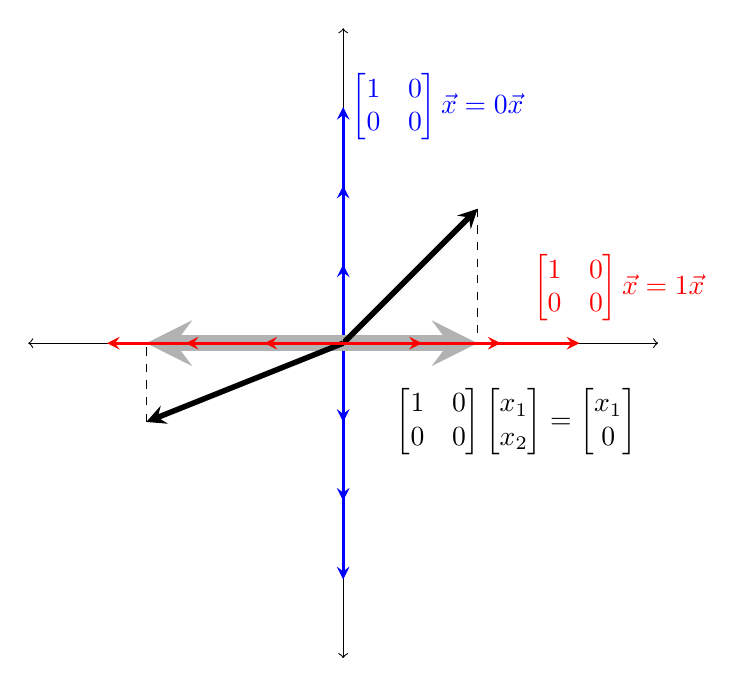
\begin{tikzpicture}

  \draw[<->] (-4,0)--(4,0);
  \draw[<->] (0,-4)--(0,4);
  
 \draw[line width=1pt,-stealth, blue](0, 0)--(0, 1);
 \draw[line width=1pt,-stealth, blue](0, 0)--(0, 2);
 \draw[line width=1pt,-stealth, blue](0, 0)--(0, 3);
 \draw[line width=1pt,-stealth, blue](0, 0)--(0, -1);
 \draw[line width=1pt,-stealth, blue](0, 0)--(0, -2);
 \draw[line width=1pt,-stealth, blue](0, 0)--(0, -3);


\draw[line width=0.5pt,dashed, black](1.707,1.707)--(1.707,0);
\draw[line width=6pt,-stealth, black!30!white](0,0)--(1.707,0);
\draw[line width=2pt,-stealth, black](0, 0)--(1.707,1.707);


\draw[line width=0.5pt,dashed, black](-2.5,-1)--(-2.5,0);
\draw[line width=6pt,-stealth, black!30!white](0,0)--(-2.5,0);
\draw[line width=2pt,-stealth, black](0, 0)--(-2.5,-1);

\draw[line width=1pt,-stealth, red](0, 0)--(-3,0);
\draw[line width=1pt,-stealth, red](0, 0)--(-2,0);
\draw[line width=1pt,-stealth, red](0, 0)--(-1,0);
\draw[line width=1pt,-stealth, red](0, 0)--(3,0);
\draw[line width=1pt,-stealth, red](0, 0)--(2,0);
\draw[line width=1pt,-stealth, red](0, 0)--(1,0);
 
 
 \node[red] at (3.5, 0.7)   (a) {$\begin{bmatrix}1&0\\0&0\end{bmatrix}\vec{x}=1\vec{x}$};
 
 \node[blue] at (1.2, 3)   (a) {$\begin{bmatrix}1&0\\0&0\end{bmatrix}\vec{x}=0\vec{x}$};

 \node[black] at (2.2, -1)   (a) {$\begin{bmatrix}1&0\\0&0\end{bmatrix}\begin{bmatrix}x_1\\x_2\end{bmatrix}=\begin{bmatrix}x_1\\0\end{bmatrix}$};
 \end{tikzpicture}
\end{image}

The blue vectors along the y-axis are also eigenvectors.  To see this, note that each of the blue vectors is of the form $\vec{x}=\begin{bmatrix}0\\x_2\end{bmatrix}$.  But then $$P\vec{x}=\begin{bmatrix}1&0\\0&0\end{bmatrix}\begin{bmatrix}0\\x_2\end{bmatrix}=\begin{bmatrix}0\\0\end{bmatrix}=0\begin{bmatrix}0\\x_2\end{bmatrix}=0\vec{x}$$
So each of the blue vectors is an eigenvector of $P$ with the corresponding eigenvalue of $0$.
\end{explanation}
\end{example}

\begin{example}\label{ex:eigsrotation}
Let $M=\begin{bmatrix}
\frac{\sqrt{2}}{2} & -\frac{\sqrt{2}}{2}\\
\frac{\sqrt{2}}{2} & \frac{\sqrt{2}}{2}
\end{bmatrix}$.  Note that $M$ takes any vector $\vec{x}$ in $\RR^2$ and rotates it $45^{\circ}$, as we saw in Example \ref{ex: rotate45} of Module LTR-M-0070.  

\begin{image}[4in]
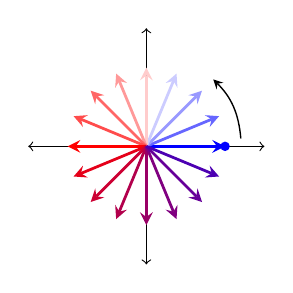
\begin{tikzpicture}

  \draw[<->] (-1.5,0)--(1.5,0);
  \draw[<->] (0,-1.5)--(0,1.5);
  
 \draw[line width=1pt,-stealth, blue](0, 0)--(1,0);
 \draw[line width=1pt,-stealth, blue!60!white](0, 0)--(0.924,0.383);
 \draw[line width=1pt,-stealth, blue!40!white](0, 0)--(0.707,0.707);
 \draw[line width=1pt,-stealth, blue!20!white](0, 0)--(0.383,0.924);
 \draw[line width=1pt,-stealth, red!20!white](0, 0)--(0,1);
 
 \draw[line width=1pt,-stealth, red!40!white](0, 0)--(-0.383,0.924);
\draw[line width=1pt,-stealth, red!60!white](0, 0)--(-0.707,0.707);
\draw[line width=1pt,-stealth, red!70!white](0, 0)--(-0.924, 0.383);
\draw[line width=1pt,-stealth, red](0, 0)--(-1,0);

\draw[line width=1pt,-stealth, red!90!blue](0, 0)--(-0.924,-0.383);
\draw[line width=1pt,-stealth, red!80!blue](0, 0)--(-0.707,-0.707);
\draw[line width=1pt,-stealth, red!70!blue](0, 0)--(-0.383,-0.924);
\draw[line width=1pt,-stealth, red!60!blue](0, 0)--(0,-1);

\draw[line width=1pt,-stealth, red!50!blue](0, 0)--(0.383,-0.924);
\draw[line width=1pt,-stealth, red!40!blue](0, 0)--(0.707,-0.707);
\draw[line width=1pt,-stealth, red!30!blue](0, 0)--(0.924,-0.383);
\fill[blue] (1,0) circle (0.06cm);

\draw [->,line width=0.5pt,-stealth]  (1.2,0.1) to[out=95, in=-45] (0.85, 0.85);
 \end{tikzpicture}
 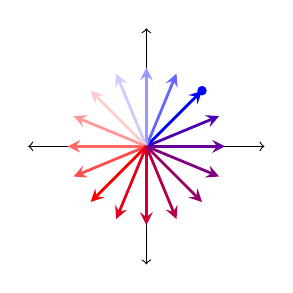
\begin{tikzpicture}
  \draw[<->] (-1.5,0)--(1.5,0);
  \draw[<->] (0,-1.5)--(0,1.5);
  
 \draw[line width=1pt,-stealth, red!40!blue](0, 0)--(1,0);
 \draw[line width=1pt,-stealth, red!30!blue](0, 0)--(0.924,0.383);
 \draw[line width=1pt,-stealth, blue](0, 0)--(0.707,0.707);
 \draw[line width=1pt,-stealth, blue!60!white](0, 0)--(0.383,0.924);
 \draw[line width=1pt,-stealth, blue!40!white](0, 0)--(0,1);
 
 \draw[line width=1pt,-stealth, blue!20!white](0, 0)--(-0.383,0.924);
\draw[line width=1pt,-stealth, red!20!white](0, 0)--(-0.707,0.707);
\draw[line width=1pt,-stealth, red!40!white](0, 0)--(-0.924, 0.383);
\draw[line width=1pt,-stealth, red!60!white](0, 0)--(-1,0);

\draw[line width=1pt,-stealth, red!70!white](0, 0)--(-0.924,-0.383);
\draw[line width=1pt,-stealth, red](0, 0)--(-0.707,-0.707);
\draw[line width=1pt,-stealth, red!90!blue](0, 0)--(-0.383,-0.924);
\draw[line width=1pt,-stealth, red!80!blue](0, 0)--(0,-1);

\draw[line width=1pt,-stealth, red!70!blue](0, 0)--(0.383,-0.924);
\draw[line width=1pt,-stealth, red!60!blue](0, 0)--(0.707,-0.707);
\draw[line width=1pt,-stealth, red!50!blue](0, 0)--(0.924,-0.383);

\fill[blue] (0.707,0.707) circle (0.06cm);
 \end{tikzpicture}
\end{image}



%{\color{red} Inserting a tikz here would be nice, I think.}

Since $M$ rotates every vector in $\RR^2$, \emph{every} nonzero vector changes direction, so there are no eigenvectors in the plane.  But it turns out that $M$ does have eigenvectors and eigenvalues, but in order to find them we need to work with vectors whose entries are complex numbers.  Since these vectors are not in $\RR^2$, we cannot see them.

%\begin{image}[3in]
%\begin{tikzpicture}

 % \draw[<->] (-4,0)--(4,0);
 % \draw[<->] (0,-4)--(0,4);
 
% \node[blue] at (0, 2)   (a) {Eigenvectors? What eigenvectors?  Nothing to see here...};

% \end{tikzpicture}
%\end{image}

%{\color{blue}I was just being goofy, do we seriously want to keep this?}

Consider the vector $\begin{bmatrix} \frac{\sqrt{2}}{2}\\ \frac{\sqrt{2}}{2} i \end{bmatrix}$.  We compute:
$$\begin{bmatrix}
\frac{\sqrt{2}}{2} & -\frac{\sqrt{2}}{2}\\
\frac{\sqrt{2}}{2} & \frac{\sqrt{2}}{2}
\end{bmatrix} \begin{bmatrix} \frac{\sqrt{2}}{2}\\ \frac{\sqrt{2}}{2} i \end{bmatrix} =
\begin{bmatrix} \frac{1}{2}-\frac{1}{2} i\\ \frac{1}{2}+ \frac{1}{2} i \end{bmatrix}= (\frac{\sqrt{2}}{2}-\frac{\sqrt{2}}{2}i) \begin{bmatrix} \frac{\sqrt{2}}{2}\\ \frac{\sqrt{2}}{2} i \end{bmatrix},$$
so $\begin{bmatrix} \frac{\sqrt{2}}{2}\\ \frac{\sqrt{2}}{2} i \end{bmatrix}$ is an eigenvector of $M$.  Its corresponding eigenvalue is $\frac{\sqrt{2}}{2}-\frac{\sqrt{2}}{2}i$.
\end{example}

We will continue to work with complex numbers as we study eigenvalues and eigenvectors.

\section{Why All the Fuss About Eigenvalues and Eigenvectors?}

\begin{remark}
The first in-depth study of eigenvalues can probably be attributed to Fourier as he studied partial differential equations early in the nineteenth century, and in particular when he studied what is known as the heat equation.\footnote{pp5-6 of Trefethen, Lloyd and Embree, Mark. Spectra and Pseudospectra. Princeton University Press, 2005.} By the twentieth century mathematicians understood the connections between differential equations and eigenvalues. Systems of differential equations are often best represented by matrices, especially in the context of using computers to find numerical solutions. Most algorithms to solve these systems work by iterating some process, and eigenvalues along with their corresponding eigenvectors indicate what will happen to such a process after many repetitions.

The most famous modern example of a large-scale eigenvalue problem is the Google PageRank algorithm, which helped set Google apart from its competitors as a search engine.  Some of the relevant mathematics can be learned by working through the paper, \href{https://doi.org/10.1137/050623280}{``The \$25,000,000,000 Eigenvector, The Linear Algebra Behind Google''}, by Kurt Bryan and Tanya Leise.  
\end{remark}

\section*{Practice Problems}

\begin{problem}Let $A=\begin{bmatrix} 2 & 1 & 1\\ 1 & 2 & 1\\ 1 & 1 & 2\end{bmatrix}$.  \begin{problem}
Show that $\begin{bmatrix} 1\\1\\1 \end{bmatrix}$ is an eigenvector of $A$.  What is its corresponding eigenvalue?
$\answer{4}$
\end{problem}
 \begin{problem}
Show that $\begin{bmatrix} 1\\-1\\0 \end{bmatrix}$ is an eigenvector of $A$.  What is its corresponding eigenvalue?
$\answer{1}$
\end{problem}
 \begin{problem}
Show that $\begin{bmatrix} 1\\1\\-2 \end{bmatrix}$ is an eigenvector of $A$.  What is its corresponding eigenvalue?
$\answer{1}$
\end{problem}
\end{problem}



\begin{problem}Let $Q=\begin{bmatrix} 0& 0\\ 0&1\end{bmatrix}$.  Note that $Q$ takes any vector in $\RR^2$ and projects it onto the $y$-axis, as we learned in Practice Problem \ref{} of Module LTR-M-0020.  Which vectors in $\RR^2$ would be eigenvectors, and what are the corresponding eigenvalues?
\end{problem}

 
\begin{problem}\label{ex:eigsrotation2}
Returning to Example \ref{ex:eigsrotation}, let $M=\begin{bmatrix}
\frac{\sqrt{2}}{2} & -\frac{\sqrt{2}}{2}\\
\frac{\sqrt{2}}{2} & \frac{\sqrt{2}}{2}
\end{bmatrix}$.  Show that $\begin{bmatrix} \frac{\sqrt{2}}{2}\\ -\frac{\sqrt{2}}{2} i \end{bmatrix}$ is an eigenvector of $M$.  What is its corresponding eigenvalue?
$\answer{\frac{\sqrt{2}}{2}+\frac{\sqrt{2}}{2}i}$
\end{problem}

%{\color{blue}I added the following problem}

\begin{problem}
Arguing geometrically, identify the linear transformation whose standard matrix has eigenvalues $\lambda_1=1$ and $\lambda_2=-1$.
\begin{multipleChoice}
\choice{Vertical Shear}
  \choice{Horizontal Shear}
  \choice{Counterclockwise Rotation through a $90^\circ$ angle}
  \choice[correct]{Reflection About the line $y=mx$}
  \choice{Horizontal Stretch}
  \choice{Vertical Stretch}
  \end{multipleChoice}
\end{problem}

\begin{problem}Let $A=\begin{bmatrix} 3&0&0\\0&3&0\\0&0&3\end{bmatrix}$.  Can you find an eigenvector and its corresponding eigenvalue?  Can you find another ``eigenpair''?  Can you find all of the eigenvectors of $A$?
\end{problem}

\begin{problem}The rotation matrix in Example \ref{ex:eigsrotation} has complex eigenvectors and eigenvalues.  Think geometrically to find an example of a (non-identity) rotation matrix with real eigenvectors and eigenvalues.

Answer:  Rotation through $\answer{180}$ degrees.
\end{problem}

\begin{problem}
Can an eigenvalue have multiple eigenvectors associated with it? 
\begin{multipleChoice}
  \choice[correct]{Yes}
  \choice{No}
    \end{multipleChoice}
    
 Can an eigenvector have multiple eigenvalues associated with it?
 \begin{multipleChoice}
  \choice{Yes}
  \choice[correct]{No}
    \end{multipleChoice}
\end{problem}

\end{document}
